\section{Caching}

\paragraph{Caching --- motivation}
\begin{items}
  \item memory (RAM) needs to be managed carefully
  \item \textbf{Ideal} properties: large, fast, nonvolatile, cheap
  \item \textbf{Real} memory: trade-offs
\end{items}

\paragraph{Caching --- cache misses}
\begin{items}
  \item \textbf{compulsory miss}: \\*
    $ - $ cold start, first reference \\*
    $ - $ data block was not cached before
  \item \textbf{capacity miss}: \\*
    $ - $ not all required data fits into cache \\*
    $ - $ accessed data previously evicted to make room for different data
  \item \textbf{conflict miss}: \\*
    $ - $ collision, interference \\*
    $ - $ depending on cache organization, data items interfere with each other \\*
    $ - $ fully associative caches are not prone to conflict misses
\end{items}

\paragraph{Caching --- Harvard architecture}
\begin{items}
  \item \textbf{principle}: separate buffer memory for data and instructions
\end{items}
\begin{figure}[H]\centering\label{CachingHarvard}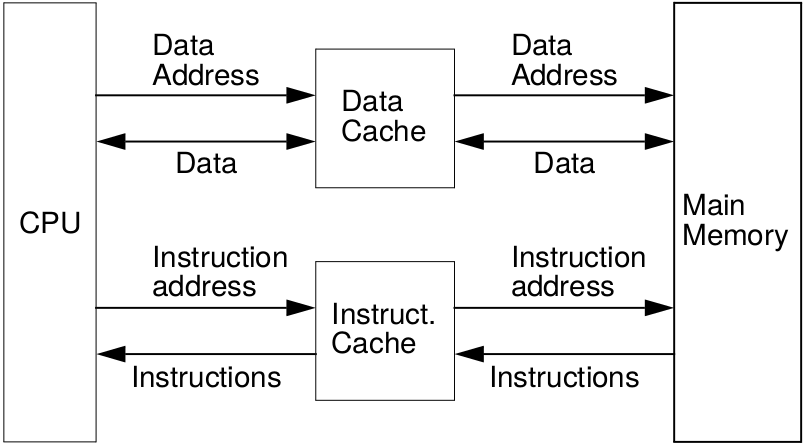
\includegraphics[width=0.33\textwidth]{CachingHarvard}\end{figure}

\paragraph{Caching --- write/replacement policies}
\begin{items}
  \item \textbf{cache hit}: \\*
    $ - $ \emph{write-through}: main memory always up-to-date, writes might be slow \\*
    $ - $ \emph{write-back}: data written only to cache, main memory temporarily inconsistent
  \item \textbf{cache miss}: \\*
    $ - $ \emph{write-allocate}: data read from main memory to cache, write performed afterwards \\*
    $ - $ \emph{write-to-memory}: modification is performed only in main memory
\end{items}

\paragraph{Cache Design Parameters}
\begin{items}
  \item \textbf{size + set size}: small cache $ \to $ set-associative implementation with large sets
  \item \textbf{line length}: spatial locality $ \to $ long cache lines
  \item \textbf{write policy}: temporal locality $ \to $ write-back
  \item \textbf{replacement policy}
  \item \textbf{tagging/indexing}: virtual or physical addresses
\end{items}

\paragraph{Caching --- problems}
\begin{items}
  \item \textbf{ambiguity problem}: same virtual addresses point to different physical addresses at different times
  \item \textbf{alias problem}: different virtual addresses point to same physical memory location
\end{items}

\paragraph{Caching --- virtually indexed, virtually tagged}
\begin{items}
  \item \textbf{operations}: \\*
    $ - $ \emph{context switch}: cache must be invalidated (and written back if write-back is used) \\*
    $ - $ \emph{fork}: child needs complete copy of parent's address space \\*
    $ - $ \emph{exec}: invalidate cache, no write-back necessary \\*
    $ - $ \emph{exit}: flush cache \\*
    $ - $ \emph{brk/sbrk}: growing = nothing, shrinking = (selective) cache invalidations
  \item \textbf{shared memory/memory-mapped files}: alias problem! \\*
    $ - $ disallow, do not cache \\*
    $ - $ only allow addresses mapping to same cache line (if using direct-mapped write-allocate cache) \\*
    $ - $ each frame accessible from exactly one virtual address at any time $ \to $ alias page invalidation
  \item \textbf{I/O}: \\*
    $ - $ \emph{buffered I/O}: no problems \\*
    $ - $ \emph{unbuffered I/O}: \\*
      \phantom{$ - $} $ \cdot $ write: information may still be in cache $ \to $ write back before I/O starts \\*
      \phantom{$ - $} $ \cdot $ read: cache must be invalidated
\end{items}
\begin{figure}[H]\centering\label{VIVT}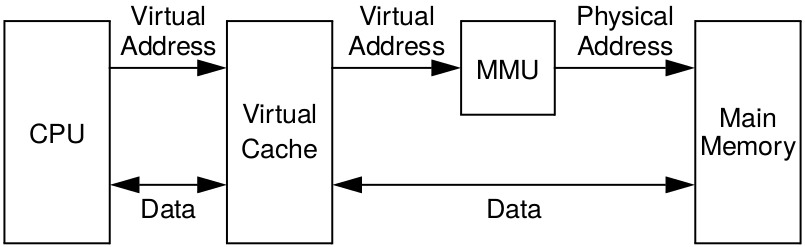
\includegraphics[width=0.33\textwidth]{VIVT}\end{figure}

\paragraph{Caching --- virtually indexed, physically tagged}
\begin{items}
  \item \textbf{usage}: often used as first-level cache
  \item \textbf{management}: \\*
    $ - $ no ambiguities \\*
    $ - $ no cache flush/context switch \\*
    $ - $ shared memory/memory mapped files: virtual starting addresses must be mapped to same \\* \phantom{$ - $} \phantom{$ \cdot $} cache line \\*
    $ - $ I/O: cache flush required
  \item \textbf{conflicts}: data structures with address distance = multiple of cache size are mapped to same line
  \item \textbf{runtime properties}: \\*
    $ - $ \emph{cache flush}: avoidable most times (fast context switches, interrupt-handling, syscalls) \\*
    $ - $ \emph{deferred write-back after context switch}: \\*
      \phantom{$ - $} $ \cdot $ avoids write accesses $ \to $ performance gain \\*
      \phantom{$ - $} $ \cdot $ variable execution time caused by compulsory misses \\*
    $ - $ \emph{dynamic memory management}: causes variable execution times through conflict misses \\*
    $ - $ \emph{multiprocessor systems}: problematic with shared memory --- which line should be invalidated? \\*
      \phantom{$ - $} $ \cdot $ cache size is small multiple of page size (1-4) \\*
      \phantom{$ - $} $ \cdot $ requires to only invalidate/flush 1-4 cache lines by cache coherency HW
\end{items}
\begin{figure}[H]\centering\label{VIPT}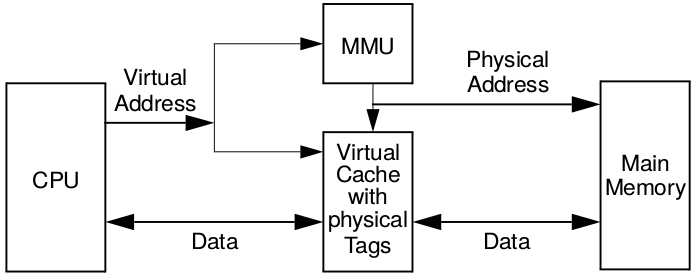
\includegraphics[width=0.33\textwidth]{VIPT}\end{figure}

\paragraph{Caching --- physically indexed, physically tagged}
\begin{items}
  \item \textbf{Advantages}: \\*
    $ - $ completely transparent to processor \\*
    $ - $ no performance-critical system support required (including I/O) \\*
    $ - $ SMPs with shared memory can use coherency protocol implemented in hardware
  \item \textbf{random allocation conflicts}: \\*
    $ - $ page conflicts caused by random allocation of physical memory \\*
    $ - $ contiguous virtual memory normally mapped to arbitrary free physical pages
  \item \textbf{random coloring conflicts}: consequences of random page coloring: \\*
    $ - $ cache conflicts \\*
    $ - $ cache only partially used \\*
    $ - $ significant runtime variations
  \item \textbf{conflict mitigation}: \\*
    $ - $ sequential page colors for individual memory segments \\*
    $ - $ \emph{cache partitioning}: divide physical memory in disjoint subsets, all pages of subset are mapped \\* \phantom{$ - $} \phantom{$ \cdot $} to same cache partition
\end{items}
\begin{figure}[H]\centering\label{PIPT}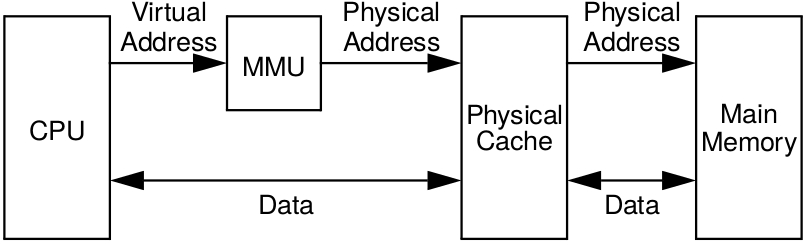
\includegraphics[width=0.33\textwidth]{PIPT}\end{figure}